%% Fig. 1 -- habit loop. Rendered to habit-loop.png by ../build-figures.sh
\documentclass[border=4pt]{standalone}
\usepackage{times}
\usepackage{tikz}
\usetikzlibrary{arrows.meta,positioning}
\newcommand{\COtwo}{CO$_2$}

\begin{document}
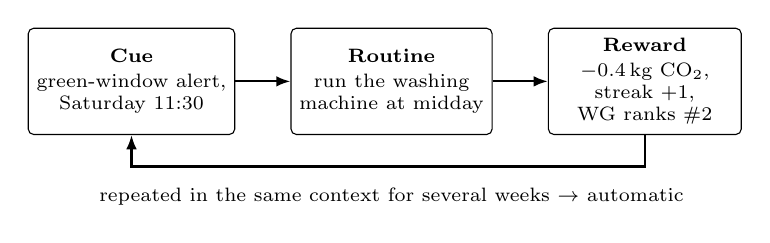
\begin{tikzpicture}[
  stage/.style={draw, rounded corners=2pt, align=center, minimum width=2.45cm,
                minimum height=1.35cm, inner sep=3pt, font=\scriptsize},
  arr/.style={-{Latex[length=1.8mm]}, thick}]
\node[stage] (cue) {\textbf{Cue}\\[1pt] green-window alert,\\ Saturday 11:30};
\node[stage, right=7mm of cue] (routine) {\textbf{Routine}\\[1pt] run the washing\\ machine at midday};
\node[stage, right=7mm of routine] (reward) {\textbf{Reward}\\[1pt] $-0.4$\,kg \COtwo,\\ streak $+1$,\\ WG ranks \#2};
\draw[arr] (cue) -- (routine);
\draw[arr] (routine) -- (reward);
% return path runs below the boxes; the label sits underneath it, not on it
\draw[arr] (reward.south) -- ++(0,-4mm) -| (cue.south);
\node[font=\scriptsize, align=center, below=5.5mm of routine.south]
  {repeated in the same context for several weeks $\rightarrow$ automatic};
\end{tikzpicture}
\end{document}
